\documentclass[landscape,usenames,dvipsnames]{sciposter}
\renewcommand{\papertype}{custom}
\renewcommand{\sectionsize}{\large}


% edit pointsize, width, height, and fontsize parameters as needed
% DO ensure that values in the \special commands match!
\usepackage[pass,paperwidth=36in,paperheight=24in]{geometry}
\renewcommand{\fontpointsize}{25pt}
\setmargins[2.5cm]

%\renewcommand{\subsectionsize}{\large \textcolor{\SectionCol}}
%\usepackage[spanish]{babel}
% or whatever
\usepackage{tikz}
\usetikzlibrary{arrows,automata,positioning}
\usepackage[latin1]{inputenc}
\usepackage{amsmath,amsthm,amssymb,bm}
\usepackage{multicol}
\usepackage{listings}
\usepackage{enumerate, wrapfig}
\usepackage{colortbl}
\usepackage[absolute]{textpos}
\usepackage{subfigure}

\usepackage{graphicx}
\graphicspath{ {images/} }

%\newcommand{\reed}[1]{\relax}
%\newcommand{\abdullah}[1]{\relax}
%\newcommand{\tatum}[1]{\relax}
%\newcommand{\eric}[1]{\relax}
%\newcommand{\christian}[1]{\relax}
%\newcommand{\Fix}[1]{\relax}
\newcommand{\reed}[1]{{\color{magenta}\bfseries [#1]}}
\newcommand{\abdullah}[1]{{\color{blue}\bfseries [#1]}}
\newcommand{\tatum}[1]{{\color{orange}\bfseries [#1]}}
\newcommand{\eric}[1]{{\color{green}\bfseries [#1]}}
\newcommand{\christian}[1]{{\color{cyan}\bfseries [#1]}}
\newcommand{\Fix}[1]{{\color{red}\bfseries [#1]}}
\newcommand{\Comment}[1]{}
\newcommand{\Space}[1]{}
\newcommand{\Num}[1]{#1}

\newcommand{\term}[1]{\emph{\textbf{#1}}}

\newcommand{\R}{\mathbb{R}}
\newcommand{\Q}{\mathbb{Q}}
\newcommand{\Z}{\mathbb{Z}}
\newcommand{\N}{\mathbb{N}}

\theoremstyle{definition}
\newtheorem{definition}{Definition}[section]
\theoremstyle{remark}
\newtheorem{remark}[definition]{Remark}
\theoremstyle{remark}
\newtheorem{example}[definition]{Example}
\theoremstyle{plain}
\newtheorem{theorem}[definition]{Theorem}
\newtheorem{conjecture}[definition]{Conjecture}

\lstdefinelanguage{pecan}{
	keywords=[1]{forall, exists, are, is},
	keywordstyle=[1]\color{blue}\bfseries,
	keywords=[2]{false, true},
	keywordstyle=[2]\color{orange}\bfseries,
	keywords=[3]{assert_prop,type},
	keywordstyle=[3]\color{teal}\bfseries,
	literate=%
	    {\#}{{{\color{teal}\bfseries\#}}}1
	    {+}{{{\color{red}+}}}1
        {:=}{{{\color{red}:=}}}1
        {..}{{{\color{red}..}}}1
        {*}{{{\color{red}*}}}1
        {:}{{{\color{red}:}}}1
        {>}{{{\color{red}>}}}1
        {<}{{{\color{red}<}}}1
        {=}{{{\color{red}=}}}1,
    escapeinside={\&}{)},
    sensitive=false, % keywords are not case-sensitive
    morecomment=[l]{//}, % l is for line comment
    morecomment=[s]{/*}{*/}, % s is for start and end delimiter
    morestring=[b]" % defines that strings are enclosed in double quotes
}


\newtheorem{thm}{Theorem}%[section] % uncomment [section] to number within section
\newtheorem*{thm*}{Theorem}
\newtheorem{lem}{Lemma}
\newtheorem{cor}[thm]{Corollary}
\newtheorem{prop}[thm]{Proposition}
\newtheorem{rem}[thm]{Remark}
\newtheorem{cond}[thm]{Condition}
\newtheorem*{namedtheorem}{Theorem}
\newtheorem*{ex}{Example}
\newtheorem*{defin}{Definition}
\newtheorem{env}[thm]{Variation}
\renewcommand {\theequation}{\arabic{section}.\arabic{equation}}

%Lines 54-73 define box theorem. You can do similar things to put boxes around conjectures, corollaries, ect, or use the mdframe to just create a box
\usepackage[framemethod=TikZ]{mdframed}
\definecolor{light-blue}{RGB}{197,219,249}
\mdfdefinestyle{MyFrame}{linecolor=light-blue,
    outerlinewidth=1.5pt,
    roundcorner=0pt,
    innertopmargin=7pt,
    innerbottommargin=7pt,
    innerrightmargin=15pt,
    innerleftmargin=15pt,
    backgroundcolor=light-blue}
\mdfdefinestyle{thmsytle}{linecolor=orange,
    outerlinewidth=2pt,
    roundcorner=20pt,
    innertopmargin=15pt,
    innerbottommargin=15pt,
    innerrightmargin=15pt,
    innerleftmargin=15pt,
    backgroundcolor=white,
	}


\mdtheorem[style=thmsytle]{MDtheorem}{Theorem}
\newcommand*{\Title}{}
\newenvironment{boxthm}[1][]{%
\refstepcounter{thm}
    \ifstrempty{#1}{\begin{MDtheorem}}%
    {\begin{MDtheorem}[(#1)]}
}{%
    \end{MDtheorem}%
}%


 
% \usepackage[
% backend=biber,
% style=alphabetic,
% sorting=ynt
% ]{biblatex}

% \addbibresource{bibliography.bib}


%\definecolor{BoxCol}{rgb}{0.9,0.9,0.9}
% uncomment for grey background to \section boxes
% for use with default option boxedsections

\definecolor{BoxCol}{rgb}{.06,.16,.28}


\definecolor{SectionCol}{rgb}{1,1,1}

\definecolor{blue}{rgb}{0,0,1}
\definecolor{orange}{rgb}{.93,.29,0.1}
\definecolor{white}{rgb}{1,1,1}

\newtheorem{Features}{Features}

%PROOFREADING DEDADLINE -- please have your parts completed by Sunday evening so that we can proofread and do last edits on Sunday night/Monday morning.


%%%%%%%%%%%%%%%%%%%%%%%%%%%%%%%%%%%%%%%%%%%%%
%title
%%%%%%%%%%%%%%%%%%%%%%%%%%%%%%%%%%%%%%%%%%%%%
\title{Automatic Theorem Proving}

\author{
Authors: Reed Oei, Eric Ma, Tatum Schmidt, Abdullah Dean \\
Graduate Mentor: Christian Schulz \\
Faculty Advisor: Philipp Hieronymi \\
}

% insert correct institute name
%\institute{University of Illinois at Urbana-Champaign}
%\email{}  shows author email address below institute

%\date is unused by the current \maketitle

%%%%%%%%%%%%%%%%%%%%%%%
% Logo for Poster
%%%%%%%%%%%%%%%%%%%%%

\leftlogo[.7]{igl-logo-small.png} % defines logo to left of title (with scale factor)
\rightlogo[.6]{imark.png} % same but on right

%%%%%%%%%%%%%%%%%%%
% Start of document
%%%%%%%%%%%%%%%%%%%
\begin{document}
%%%%%%%%%%%%%%%%%%%%%%
%% Poster Set up
%%%%%%%%%%%%%%%%%%%%%%%
\conference{IGL Poster Session Fall 2019}% you can change this for other conferences

\maketitle
\vspace{-3ex}
\begin{multicols}{3}  % sets up 3 column poster



%%%%%%%%%%%%%%%%%%%%%%
%% Start of First Column
%%%%%%%%%%%%%%%%%%%%%%%
%Sections have a color box around them. Remove the * if you want to number your sections
\section*{Introduction}
\begin{mdframed}[style=MyFrame]
\subsection*{Automated Theorem Proving}
\end{mdframed}

An \textbf{automated theorem prover} is a program that takes as input a statement and \emph{decides} (i.e., proves or disproves) it. 
Theorem provers can be very useful: computers are reliable, and they never get tired or bored, allowing us to quickly explore new ideas.
Though it is impossible to decide \emph{all} statements, we can still use theorem provers to solve many interesting problems. 

\begin{mdframed}[style=MyFrame]
\subsection*{Automata}
\end{mdframed}
A \textbf{finite automaton} is a ``machine'' that accepts some \textbf{finite word}, or string of letters, such as ``abc.'' A finite automaton can be represented as a \emph{finite} collection of \textbf{states} and \textbf{transitions}.

\vspace{-15mm}
\begin{figure}
    \centering
    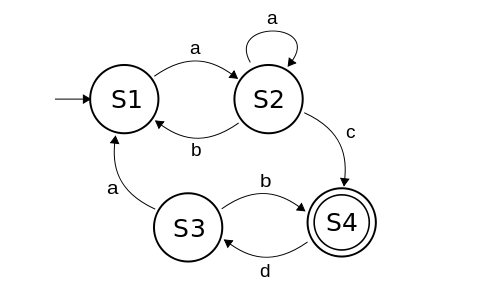
\includegraphics[width=.50\textwidth]{images/Automata.png}
    \caption{An automaton that accepts ``aac'' and rejects ``ab'' and ``caa''.}
    \label{fig:aut_example}
\end{figure}
\vspace{-20mm}


\begin{mdframed}[style=MyFrame]
\subsection*{Closure Properties of Automata}
\end{mdframed}
Automata have closure properties: we can combine them using first-order logic operations.
% \begin{thm}
% Suppose automaton $A$ accepts language $L(A)$ and automaton $B$ accepts language $L(B)$, then there exists, and we can construct, automata that accepts $L(A)\cup L(B)$, $L(A) \cap L(B)$, and  $\overline{L(A)}$.
% \end{thm}
\begin{thm}
    Suppose we have predicates $P$ and $Q$, such that automaton $\mathcal{A}$ accepts words that makes $P$ true, and $\mathcal{B}$ accepts words that makes $Q$ true, then we can construct, from $\mathcal{A}$ and $\mathcal{B}$, the automata that accepts words that makes $P \land Q$, $P \lor Q$, $\lnot P$ true.
\end{thm}

\vspace{-15mm}
\begin{figure}[h]
    \subfigure[]{\label{fig:eventually_zero}%
        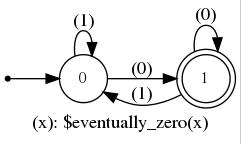
\includegraphics[width=0.3\linewidth]{images/eventually_zero.jpg}%
    }
    \subfigure[]{\label{fig:even_ones}%
        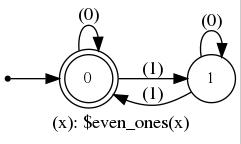
\includegraphics[width=0.3\linewidth]{images/even_ones.jpg}%
    }
    \subfigure[]{\label{fig:both}%
        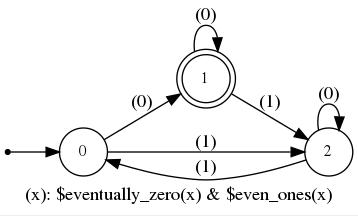
\includegraphics[width=0.3\linewidth]{images/both.jpg}%
    }
    % How to do subreferences?
    \caption{Demonstrating the closure properties: (c) is formed by ``and-ing'' (a) and (b)}
\end{figure}
\vspace{-20mm}

For the quantifiers, $\forall$ and $\exists$, we need to define automata that accepts multiple inputs. 
\begin{defin}
    An automaton $\mathcal{A}$ accepts a pair of words $ (x_1x_2\dots x_n, y_1y_2\dots y_n)$ if it accepts the word $(x_1,y_1)(x_2,y_2)\dots(x_n,y_n)$.
\end{defin}
\begin{thm}
    Suppose $p(x,y)$ is a predicate with two inputs, and automaton $\mathcal{A}$ accepts pairs of words that makes $p$ true, then we can construct an automaton, from $\mathcal{A}$, which accepts words that makes $p'(y) = \exists x. p(x,y)$ true.
\end{thm}
% Therefore, we can combine predicates using first-order quantifiers and construct the automaton associated with the predicate.

\textbf{B\"uchi Automata} are an extension of finite automata to infinite inputs; they accept words that visit an accepting state infinitely often. 
Using B\"uchi automata has a number of advantages:
\begin{itemize}
        \item Some problems are more naturally expressed with B\"uchi automata
        \item Some problems can \emph{only} be expressed with B\"uchi automata
        \item We can still express properties about finite strings
\end{itemize}
% A major application of B\"uchi automata is in model checking: verifying that programs have the expected behavior.

\columnbreak

%%%%%%%%%%%%%%%%%%%%%%%%%%%%%%%%%%%%%
%% New Section
%%%%%%%%%%%%%%%%%%%%%%%%%%%%%%%%%%%%%
\section*{Pecan: A Theorem Prover}

\textbf{Pecan} is a system for automated theorem proving that represents logical predicates using B\"uchi automata.
Pecan programs are made up of \textbf{predicates} and \textbf{directives}:

\begin{itemize}
    \item predicates: defined either by loading automata defined in files, translating LTL (linear temporal logic) formulas into B\"uchi automata, or some combination of these using first order logic and equality.

\begin{lstlisting}[language=pecan, basicstyle=\normalsize\ttfamily, mathescape=true, frame=single]
eq_sym() := $\forall$x. $\forall$y. x =$\ $y $\color{red} \iff$ y =$\ $x
\end{lstlisting}

    \item directives: commands to the Pecan interpreter, such as: \texttt{assert\_prop}, which asks Pecan to prove a theorem, or \texttt{save\_aut}, which asks Pecan to build the automaton corresponding to some predicate and save it to a file
    
\begin{lstlisting}[language=pecan, basicstyle=\normalsize\ttfamily, mathescape=true, frame=single]
#assert_prop(true, eq_sym)
\end{lstlisting}

\end{itemize}

The Pecan language is a statically-typed, interpreted programming language.
The basic datatype, or universal set, in Pecan is the infinite binary word---elements of $\Sigma^{\omega}$ where $\Sigma = \{0,1\}$.
All types are \textbf{refinement types}: they are defined as a subset of $\Sigma^{\omega}$ satisfying some predicate defined in terms of B\"uchi automata.

\begin{ex}
A word $x \in \Sigma^\omega$ has type \texttt{binary} if $x \in \{ w \in \Sigma^* : x = w0^\omega \}$---that is, binary words that are eventually $0$.

Equivalently, we can define $\texttt{binary}$ as the words satisfying the LTL formula $F(G(\neg x))$.
\end{ex}

Users can define their own \textbf{structures} on a type so that names can be overloaded: for example, this allows users to define their own numeration systems.

\begin{lstlisting}[language=pecan, basicstyle=\normalsize\ttfamily, mathescape=true, frame=single]
#type(binary, {
    "adder": bin_add(any, any, any),
    "less": bin_less(any, any) 
})
\end{lstlisting}

Pecan is capable of proving any statement expressed solely in terms of B\"uchi automata and first order logic connectives, such as $\wedge$, $\vee$, $\neg$, $\forall$, and $\exists$.
In particular, it is powerful enough to decide any statement in Presburger arithmetic, the first order theory of the natural numbers with addition (but \emph{not} multiplication) and comparison.

\begin{mdframed}[style=MyFrame]
\subsection*{Example: The Chicken McNugget Problem }
\end{mdframed}

In the 1980s, Henri Picciotto asked the following problem in his algebra textbook:

\begin{quote}
    What is the greatest number of chicken nuggets that cannot be ordered using only boxes of 6, 9, and 20?
\end{quote}

We call all such numbers \textbf{non-purchasable}, and we can define them in Pecan as follows:

\begin{lstlisting}[language=pecan, basicstyle=\normalsize\ttfamily, mathescape=true, frame=single]
n,m,a,b,c $\color{red} \in$ binary
purchasable(n) := n $\color{red} \in$ binary $\color{red} \wedge$ $\exists$a. $\exists$b. $\exists$c. n =$\ $6*a $\color{red} +$ 9*b $\color{red} +$ 20*c
non_purchasable(n) := n $\color{red} \in$ binary $\color{red} \wedge$ $\color{red} \neg$purchasable(n)
\end{lstlisting}

We can then define the largest non-purchasable number naturally as:
\begin{lstlisting}[language=pecan, basicstyle=\normalsize\ttfamily, mathescape=true, frame=single]
largest(n) := non_purchasable(n) $\color{red} \wedge$ $\forall$m $\color{red} \in$ non_purchasable. n $\color{red} \geq$ m
\end{lstlisting}

Pecan produces the automaton in Figure~\ref{fig:largest_non_purchasable} for us, which tells us that the largest non-purchasable number is $101011_2$, or $43$ in base 10.

\begin{figure}
    \centering
    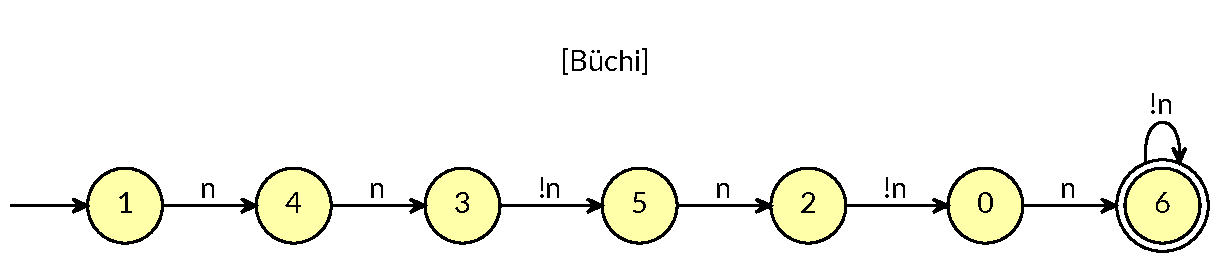
\includegraphics[width=\textwidth]{images/largest_not_purchasable.pdf}
    \caption{A B\"uchi automaton accepting $110101$ in least significant digit first representation.}
    \label{fig:largest_non_purchasable}
\end{figure}

\columnbreak

\begin{mdframed}[style=MyFrame]
\subsection*{Example: Properties of the Thue-Morse Word}
\end{mdframed}

Below is an example of a Pecan program which proves two well-known properties of the Thue-Morse word, $T$, which is defined by: the $n$-th digit of the Thue-Morse word, $T[n]$, is $1$ if the binary representation of $n$ has an odd number of $1$'s, and $0$ otherwise.

The Thue-Morse word starts with: {\Large\[ 01101001100101101001011001101001\dots  \]}
\begin{defin}
    A word $w$ is a \textbf{square} if it is of the form $w = xx$ for some nonempty word $x$.
    Similarly, $w$ is a \textbf{cube} if it is of the form $w = xxx$ for some nonempty word $x$.
\end{defin}

\begin{thm}
    The Thue-Morse word contains squares, but does not contain any cubes.
\end{thm}

Here is the equivalent definition of $T$ in Pecan (\texttt{odd\_ones} is defined as an automaton):
\begin{lstlisting}[language=pecan, basicstyle=\normalsize\ttfamily, mathescape=true, frame=single]
T(x) := odd_ones(x)
\end{lstlisting}

Below are definitions of square and cube for the Thue-Morse word in Pecan.

\begin{lstlisting}[language=pecan, basicstyle=\normalsize\ttfamily, mathescape=true, frame=single]
i,j,n $\color{red} \in$ binary
square(i, n) := n > 0 $\color{red} \wedge$ T[i $\color{red} \ldots$ i+n] =$\ $T[i+n $\color{red} \ldots$ i+2*n]
cube(i, n) := square(i, n) $\color{red} \wedge$ square(i+n, n)
\end{lstlisting}

Finally, we state the theorems we would like to prove, and ask Pecan to attempt to prove that there are squares, but there are no cubes.

\begin{lstlisting}[language=pecan, basicstyle=\normalsize\ttfamily, mathescape=true, frame=single]
squares_exist() := $\exists$i. $\exists$n. square(i, n)
#assert_prop(true, squares_exist)
cubes_exist() := $\exists$i. $\exists$n. cube(i, n)
#assert_prop(false, cubes_exist)
\end{lstlisting}

The output from Pecan is the following, indicating that the theorem is true.
\begin{lstlisting}[basicstyle=\normalsize\ttfamily, mathescape=true, frame=single]
[INFO] Checking if squares_exist is true.
$\text{\color{ForestGreen}squares\_exist is true.}$
[INFO] Checking if cubes_exist is false.
$\text{\color{ForestGreen}cubes\_exist is false.}$
\end{lstlisting}

Here is another theorem about the Thue-Morse word that we can check.
\begin{thm}
There are no overlapping squares, i.e. words of form $0x0x0$ or $1x1x1$ for some nonempty word $x$. 
\end{thm}
We can check it by running the following Pecan commands.

\begin{lstlisting}[language=pecan, basicstyle=\normalsize\ttfamily, mathescape=true, frame=single]
i,j,n $\color{red} \in$ binary
o_square(i, n) := n > 0 $\color{red} \wedge$ T[i+1 $\color{red} \ldots$ i+n+1] = $\ $T[2+i+n $\color{red} \ldots$ 2+i+2*n] $\color{red} \wedge$  T[i] =$\ $T[i+n] $\color{red} \wedge$ T[i] =$\ $T[2+i+2*n]
o_squares_exist() := $\exists$i. $\exists$n. o_square(i, n)
#assert_prop(false, o_squares_exist)
\end{lstlisting}
Pecan verifies the theorem: 
\begin{lstlisting}[basicstyle=\normalsize\ttfamily, mathescape=true, frame=single]
[INFO] Checking if o_squares_exist is false.
$\text{\color{ForestGreen} o\_squares\_exist is false.}$
\end{lstlisting}

\section*{Future Work}

\begin{itemize}
\item Continue to develop Pecan and write a manual for it Pecan. 
\item Previously, we proved various theorems about special classes of Sturmian words. Using Pecan we hope to prove theorems about all Sturmian words at once.
\item Since Pecan uses B\"uchi automata, which accept infinite words, we can represent sets of real numbers using B\"uchi automata and prove properties about the real numbers.
\end{itemize}

\vspace*{-10pt}  %change to -10
\section*{References}

{\footnotesize [1] Khoussainov, Bakhadyr.Nerode, Anil. (2001) \emph{Automata Theory and its Applications}, MA : Birkh\"auser Boston
}
% \eric{I guess we don't need reference 2,3,4. But any other references that we need?}
% {\footnotesize [2] Rampersad, Narad. Shallit, Jeffrey and  Vandomme, Elise. (2018) \emph{Critical exponents of infinite balanced words}, Canada
% }

% {\footnotesize [3] Du, Chen Fei. Mousavi, Hammoon. Schaeffer, Luke and Shallit, Jeffrey. (2014) \emph{Decision Algorithms for Fibonacci-Automatic Words, with Applications to Pattern Avoidance}
% }

% {\footnotesize [4] Hieronymi, P., \& Terry Jr, A. (2018). \emph{Ostrowski Numeration Systems, Addition, and Finite Automata}. Notre Dame Journal of Formal Logic, 59(2), 215-232.
% }

\vspace*{10mm} %This will change to -5
\emph{
Support for this project was provided by the Illinois Geometry Lab and the Department of Mathematics at the University of Illinois at Urbana-Champaign.
}
\end{multicols}

\end{document}
